\begin{figure}
	\centering
	%\tikzset{external/remake next}
	\begin{tikzpicture}[spy using outlines={rectangle, red, magnification=6,
		size=3.8cm, connect spies}]
		\node{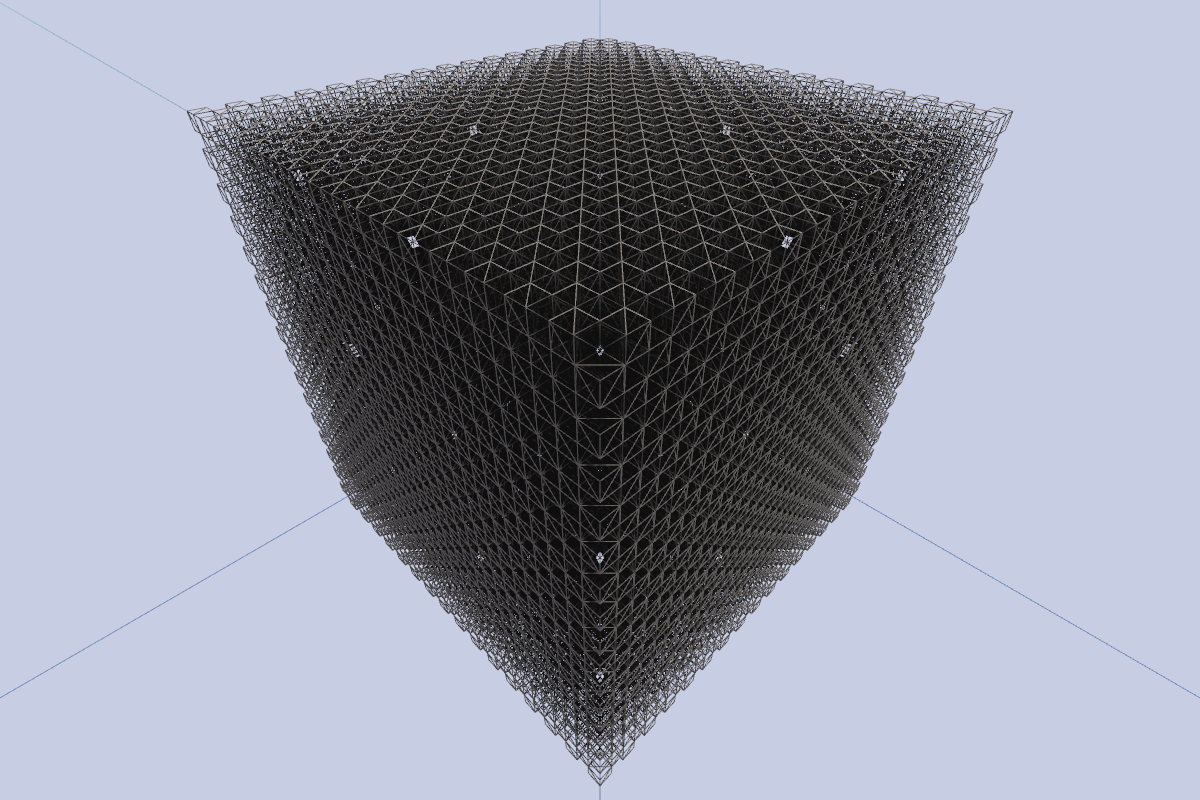
\includegraphics[width=.7\textwidth]{fps-cube.png}};
		\spy on (-3.8,2.65) in node [right] at (-10,2);
		\spy on (0.25,.65) in node [right] at (-10,-2);
	\end{tikzpicture} 
	\caption[Screenshot der Blockformation in Szenario 2: Halb-Würfel.]{Screenshot der Blockformation in Szenario 2: Halb-Würfel. Es wird das Gitternetz der Blöcke dargestellt, um die Menge der angezeigten Elemente zu maximieren. Zur besseren Ansicht sind zwei Bereiche vergrößert dargestellt. Links unten ist die Zerteilung der Würfelseiten in je zwei Dreiecke zu erkennen. Links oben wird ersichtlich, dass das Gitternetz tatsächlich nur die Kanten der Dreiecke zeichnet. Der Rest der Seiten ist durchsichtig.}\label{fig:cube}
\end{figure}
Da die Anzahl der zu zeichnenden Objekte in dem ersten Szenario relativ gering ist, wird diese in Szenario 2, das in Abbildung~\ref{fig:cube} veranschaulicht ist, erhöht. In diesem Szenario wird ein Bereich von $32 \times 32 \times 32$ Blöcken so befüllt, dass an jeder zweiten Stelle ein Block ist. Zweidimensional entspricht das einem Schachbrettmuster. Die Anzahl der platzierten Blöcke ist damit $\frac{1}{2}\cdot32^3 = 16384$. Die Anzahl der zu zeichnenden Dreiecke ist $16384\cdot6 + 5 = 98309$.

Aufgrund der Anordnung wären allerdings nur wenige Blöcke sichtbar. Daher wird das Drahtgittermodell gezeichnet, also nur die Kanten der zu zeichnenden Dreiecke. Dennoch kann hier nicht mehr sichergestellt werden, dass auch tatsächlich alle Elemente gezeichnet werden, da selbst mit dem Drahtgittermodell an vielen Stellen Polygone überdeckt werden. Durch die Darstellung als Drahtgittermodell lassen sich nun auch die Kanten der Skybox erkennen und man sieht, dass das Dreiecke in der oberen rechten Ecke nicht gezeichnet wird. 


\paragraph{\ac{fps}}Der Verlauf der Framerate für Szenario 2 ist in Abbildung~\ref{fig:seed-0-cube-fps} dargestellt.
In SystemA werden Frames ab Sekunde $11$ erzeugt, in SystemB ab Sekunde $13$. Die mittlere Framerate in SystemA ist \SI{253}{\fps} und in SystemB \SI{417}{\fps}. Damit erhöht sich die Framerate in SystemB um \SI{65}{\percent}. Dieser Wert ist deutlich geringer als in Szenario 1. Die Frameraten bleiben in beiden Systemen sehr konstant.
\begin{figure}[!htb]
	\fpsplot{seed-0-cube}
	\caption{Graph des Verlaufs der Framerate in Szenario 2: Halb-Würfel.}\label{fig:seed-0-cube-fps}
\end{figure}

\paragraph{\ac{cpu}} Die Auslastung der \ac{cpu} in Szenario 2, zu sehen in Abbildung~\ref{fig:seed-0-cube-cpu}, gestaltet sich vergleichbar zu der in Szenario 1. Die Mittelwerte sind mit \SI{13}{\percent} in SystemA und \SI{18}{\percent} in SystemB nach Rundung identisch zu Szenario 1.
\begin{figure}[!htb]
	\cpuplot{seed-0-cube}
	\caption[Graph des Verlaufs der \glsentryshort{cpu}-Auslastung in Szenario 2: Halb-Würfel.]{Graph des Verlaufs der \ac{cpu}-Auslastung in Szenario 2: Halb-Würfel.}\label{fig:seed-0-cube-cpu}
\end{figure}
Auffällig ist, dass SystemB wie in Szenario 1 in den ersten Sekunden, während des Starts der Blocklib, zwei Auslastungsspitzen besitzt (\SI{32}{\percent} und \SI{50}{\percent}). SystemA dagegen besitzt nur eine (\SI{46}{\percent}). Eine mögliche Erklärung dafür ist die Trennung von Simulation und Rendering in verschiedene Threads. Dadurch könnte es passieren, die \ac{cpu} zeitweise dadurch entlastet ist, dass die \ac{gpu} Zeit benötigt, um übergebene \glspl{Anweisung} auszuführen, beispielsweise wenn Texturen zum Start auf die \ac{gpu} geladen werden.

\paragraph{\ac{gpu}} Die \ac{gpu}-Auslastung des Halb-Würfel Szenario unterscheidet sich im Gegensatz zur \ac{cpu}-Auslastung sehr von der im Hexagon-Szenario gemessenen. In Abbildung~\ref{fig:seed-0-cube-gpu} ist die gemessene \ac{gpu}-Auslastung zeitlich aufgetragen. 
\begin{figure}[!htb]
	\gpuplot{seed-0-cube}
	\caption[Graph des Verlaufs der \glsentryshort{gpu}-Auslastung in Szenario 2: Halb-Würfel.]{Graph des Verlaufs der \ac{gpu}-Auslastung in Szenario 2: Halb-Würfel.}\label{fig:seed-0-cube-gpu}
\end{figure}
Anders als in Szenario 1 ist in beiden Systemen der Unterschied in der Auslastung unübersehbar. SystemB nutzt nach dem Start durchschnittlich \SI{94}{\percent} der Leistung der \ac{gpu}, während SystemA nur \SI{60}{\percent} Auslastung erzeugt. Über die gesamte Messdauer liegt SystemB damit bei \SI{70}{\percent} Auslastung und SystemA bei \SI{45}{\percent}. Betrachtet man nur die Auslastung nach dem Start lässt sich eine Steigerung der Auslastung um \SI{57}{\percent} errechnen.

\begin{figure}[!htb]
	\memplot{seed-0-cube-single-mem.csv}
	\memplot{seed-0-cube-multi-mem.csv}
	\caption{Graph des Verlaufs der Speichernutzung in Szenario 2: Halb-Würfel.}\label{fig:seed-0-cube-mem}
\end{figure} 
\paragraph{\ac{ram}} Die Speichernutzung in Szenario 2 wird in Abbildung~\ref{fig:seed-0-cube-mem} gezeigt. Der Ge\-samt-Spei\-cher\-ver\-brauch von SystemA steigt im Vergleich zum Hexagon-Szenario leicht während der Speicherverbrauch von SystemB beinahe identisch bleibt. SystemA benötigt durchschnittlich \SI{643}{\mega\byte} und SystemB \SI{941}{\mega\byte}. Das ist ein Anstieg von \SI{12}{\percent} in SystemA und eine leichte Verringerung um \SI{1}{\percent} in SystemB. Weiterhin zeigt SystemB einen großen Speicherverbrauch während des Starts der Blocklib (\SI{1732}{\mega\byte}).

Die Speichernutzung der kurzlebigen Objekte ist sowohl in SystemA mit \SI{53}{\mega\byte\per\second} als auch in SystemB mit \SI{101}{\mega\byte\per\second} niedriger als in Szenario 1. Insbesondere SystemB verbraucht mit neu erzeugten Objekten weniger als halb so viel Speicher. Vergleicht man die beiden Systeme in diesem Szenario erhält man einen Anstieg von \SI{91}{\percent} Speicherverbrauch mit SystemB. Der geringere Speicherverbrauch führt auch zu einer geringeren Anzahl an Garbage Collections. Da SystemB allgemein mehr Speicher nutzt als SystemA ist die Anzahl der Garbage Collections im gemessenen Zeitraum in SystemB mit 10 Collections um eins niedriger als in SystemA. Der zusätzliche Speicher gleicht also den höheren dauerhaften Speicherverbrauch aus. 

Der langlebige Speicherverbrauch bleibt in beiden Systemen mit \SI{296}{\mega\byte} (SystemA) und \SI{320}{\mega\byte} (SystemB) sehr konstant. In SystemA sinkt der Speicherverbrauch, wie auch schon im Hexagon-Szenario zu beobachten, nach etwa \SI{45}{\second} auf zum Ende hin nur noch \SI{129}{\mega\byte}.